%%%%%%%%%%%%%%%%%%%%%%%%%%%%%%%%%%%%%%%%%
% MUW Poster
% LaTeX Template
% Version 1.0 (31/08/2016)
% (Based on Version 1.0 (31/08/2015) of the Jacobs Portrait Poster
%
% License:
% CC BY-NC-SA 3.0 (http://creativecommons.org/licenses/by-nc-sa/3.0/)
%
% Created by:
% Nicolas Ballarini, CeMSIIS, Medical University of Vienna
% nicoballarini@gmail.com
% http://statistics.msi.meduniwien.ac.at/
%%%%%%%%%%%%%%%%%%%%%%%%%%%%%%%%%%%%%%%%%


\def\footer#1{\def\insertfooter{#1}}
%--------------------------------------------------------------------------------------
%	PACKAGES AND OTHER DOCUMENT CONFIGURATIONS
%--------------------------------------------------------------------------------------

\documentclass[final]{beamer}



\usepackage[scale=1.150]{beamerposter} % Use the beamerposter package
\usetheme{MUWposter} % Use the MUWposter theme supplied with this template

% Include a logo of your project if desired
\logo{\pgfputat{\pgfxy(-11,107)}{\pgfbox[center,base]{
\includegraphics[width=7cm]{ProjectLogo.png}}}}  

\usepackage{multicol}
\usepackage{array}
%The following two are column definitions for the aknowledgements section
\newcolumntype{L}{>{\arraybackslash}m{22cm}}
\newcolumntype{S}{>{\arraybackslash}m{5cm}}
\usepackage{pgf}  
\usepackage{mathtools}
\usepackage{amsmath, amsthm, amssymb, amsfonts}
\usepackage{exscale}
\usepackage{xcolor}
\usepackage{ushort}
\usepackage{setspace}
\usepackage[square,numbers]{natbib}
\usepackage{url}
\bibliographystyle{abbrvnat}
\renewcommand{\vec}[1]{\ushort{#1}}
\renewcommand{\vec}[1]{\mathbf{#1}}
\definecolor{greenMUW}{RGB}{60,191,174}
\definecolor{blueMUW}{RGB}{17,29,79}
\definecolor{skinMUW}{RGB}{254,228,217}
\definecolor{hellblauMUW}{RGB}{95,180,229}

%-----------------------------------------------
%  START Set the colors
%  Uncomment to apply colors you want to use.
%-----------------------------------------------
\colorlet{themecolor}{greenMUW}
\usebackgroundtemplate{
\includegraphics{MUW_green.pdf}}

%\colorlet{themecolor}{skinMUW}
%\colorlet{themecolor}{blueMUW}
%\usebackgroundtemplate{
\includegraphics{MUW_skin.pdf}}

%%\colorlet{themecolor}{blueMUW}
%\colorlet{themecolor}{hellblauMUW}
%\usebackgroundtemplate{
\includegraphics{MUW_hellblau.pdf}}
%-----------------------------------------------
%  END Set the colors
%-----------------------------------------------


%-----------------------------------------------
%  START Set the width of the columns
%-----------------------------------------------
\setlength{\paperwidth}{33.1in} % A0 width: 46.8in
\setlength{\paperheight}{46.8in} % A0 height: 33.1in
\newlength{\sepmargin}
\newlength{\sepwid}
\newlength{\onecolwid}
\newlength{\twocolwid}
\newlength{\threecolwid}

% The following measures are used for 2 columns
\setlength{\sepmargin}{0.055\paperwidth} % Separation width (white space) between columns
\setlength{\sepwid}{0.03\paperwidth} % Separation width (white space) between columns
\setlength{\onecolwid}{0.43\paperwidth} % Width of one column
\setlength{\twocolwid}{0.9\paperwidth} % Width of two columns

%-----------------------------------------------------------
% The following measures are used for 3 columns
%\setlength{\sepmargin}{0.06\paperwidth} % Separation width (white space) between columns
%\setlength{\sepwid}{0.02\paperwidth} % Separation width (white space) between columns
%\setlength{\onecolwid}{0.28\paperwidth} % Width of one column
%\setlength{\twocolwid}{0.58\paperwidth} % Width of two columns
%\setlength{\threecolwid}{0.88\paperwidth} % Width of three columns
%\setlength{\columnsep}{30pt}

%-----------------------------------------------
%  END Set the width of the columns
%-----------------------------------------------


%--------------------------------------------------------------------------------------
%	TITLE SECTION 
%--------------------------------------------------------------------------------------
\setbeamertemplate{title}[left]
\setbeamertemplate{frametitle}[default][left]
%\setmainfont{Georgia}

\title{Titel des Posters, Schriftgröße variabel} % Poster title

\author{AutorInnen, Schriftgröße variabel} % Author(s)

\institute{Klinik, Medizinische Universität Wien, Schriftgröße variabel} % Institution(s)
%--------------------------------------------------------------------------------------



\begin{document}

  \addtobeamertemplate{block end}{}{\vspace*{1ex}} % White space under blocks
  \addtobeamertemplate{block alerted end}{}{\vspace*{0ex}} % White space under highlighted (alert) blocks
  \setlength{\belowcaptionskip}{2ex} % White space under figures
  \setlength\belowdisplayshortskip{1ex} % White space under equations
  
  
  \begin{frame}[t] % The whole poster is enclosed in one beamer frame

      \begin{columns}[t] % The whole poster consists of two major columns
	  
      \begin{column}{\sepmargin}\end{column}
      
	    \begin{column}{\onecolwid} % The first column


		  \begin{block}{Objective}
          %\begin{multicols}{2}
          Uptam, offictibus rem vendipici nonsecest la cullabor moluptas exero quo blam quamentum repudistiam iunda doluptate dolorecta quatem faceaquodit optatum nonse init volori doluptas nam erferch ilique comnihil ma doluptate sanditat ommo temquia nonse sed modicium que vollacillab ius. Uptam, offictibus rem vendipici nonsecest la cullabor moluptas exero quo blam.
          %\end{multicols}
          \end{block}
          
          \begin{block}{Patients and Methods}
          %\begin{multicols}{2}
          Uptam, offictibus rem vendipici nonsecest la cullabor moluptas exero quo blam quamentum repudistiam iunda doluptate dolorecta quatem faceaquodit optatum nonse init volori doluptas nam erferch ilique comnihil ma doluptate sanditat ommo temquia nonse sed modicium que vollacillab ius. Uptam, offictibus rem vendipici nonsecest la cullabor moluptas exero quo blam.
Uptam, offictibus rem vendipici nonsecest la cullabor moluptas exero quo blam quamentum repudistiam iunda doluptate dolorecta quatem faceaquodit optatum nonse init volori doluptas nam erferch ilique comnihil ma doluptate sanditat ommo temquia nonse sed modicium que vollacillab ius.
          %\end{multicols}
          \end{block}
          
          \begin{table}[ht]
					\centering
					\begin{tabular}{lccc}
                    Patient Characteristics & n 		& & \%  \\
					\hline
					Total of Patients 		& 100     	& & 100 \\
					Age 	 				&  45      	& &  45 \\
					Gender 					&  50 	   	& &  50 \\
				    \hline
				  \end{tabular}
				\caption{Considered scenarios} 
                \label{Patient and tumor Characteristics}
			  \end{table}
          
          
          \begin{block}{Results}
          %\begin{multicols}{2}
          Uptam, offictibus rem vendipici nonsecest la cullabor moluptas exero quo blam quamentum repudistiam iunda doluptate dolorecta quatem faceaquodit optatum nonse init volori doluptas nam erferch ilique comnihil ma doluptate sanditat ommo temquia nonse sed modicium que vollacillab ius. Uptam, offictibus rem vendipici nonsecest la cullabor moluptas exero quo blam.
Uptam, offictibus rem vendipici nonsecest la cullabor moluptas exero quo blam quamentum repudistiam iunda doluptate dolorecta quatem faceaquodit optatum nonse init volori doluptas nam erferch ilique comnihil ma doluptate sanditat ommo temquia nonse sed modicium que vollacillab ius. 
blam quamentum repudistiam iunda doluptate dolorecta quatem faceaquodit optatum nonse init volori doluptas nam erferch ilique comnihil ma doluptate sanditat ommo temquia nonse sed modicium que vollacillab ius. Uptam, offictibus rem vendipici nonsecest la cullabor moluptas exero quo blam.

          %\end{multicols}
          \end{block}
          
          
          \begin{block}{Conclusion}
          %\begin{multicols}{2}
          Uptam, offictibus rem vendipici nonsecest la cullabor moluptas exero quo blam quamentum repudistiam iunda doluptate dolorecta quatem faceaquodit optatum nonse init volori doluptas nam erferch ilique comnihil ma doluptate sanditat ommo temquia nonse sed modicium que vollacillab ius. Uptam, offictibus rem vendipici nonsecest la cullabor moluptas exero quo blam.
          %\end{multicols}
          \end{block}
          
         \end{column}
                  
                  
                  
         \begin{column}{\sepwid}  \end{column}
         
         
         
         
         \begin{column}{\onecolwid} %The second column
         
         \begin{block}{\vspace*{2.7cm}}
          %\begin{multicols}{2}
          Uptam, offictibus rem vendipici nonsecest la cullabor moluptas exero quo blam quamentum repudistiam iunda doluptate dolorecta quatem faceaquodit optatum nonse init volori doluptas nam erferch ilique comnihil ma doluptate sanditat ommo temquia nonse sed modicium que vollacillab ius. Uptam, offictibus rem vendipici nonsecest la cullabor moluptas exero quo blam.
          %\end{multicols}
          \end{block}
          
          \begin{block}{ }
				\begin{figure}
                	\vspace*{-1cm}
                    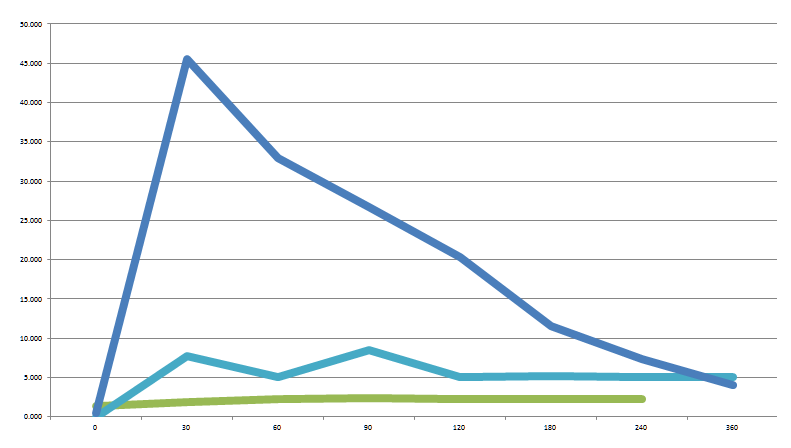
\includegraphics[width=.9\linewidth]{plot.PNG}
				\end{figure}
				\begin{figure}
                    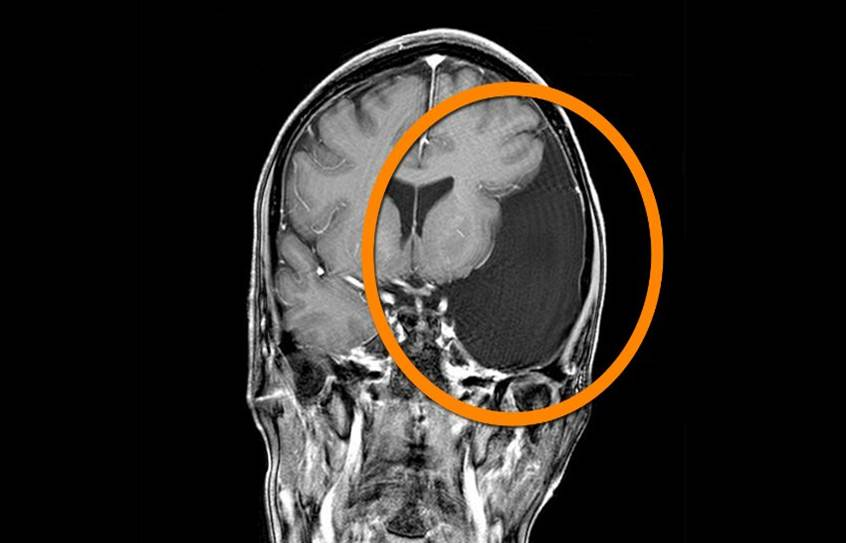
\includegraphics[width=.9\linewidth]{Bild1.jpg}
				\end{figure}
                
                \begin{multicols}{2}
                \begin{figure}
                	\vspace*{-0.95cm}
                    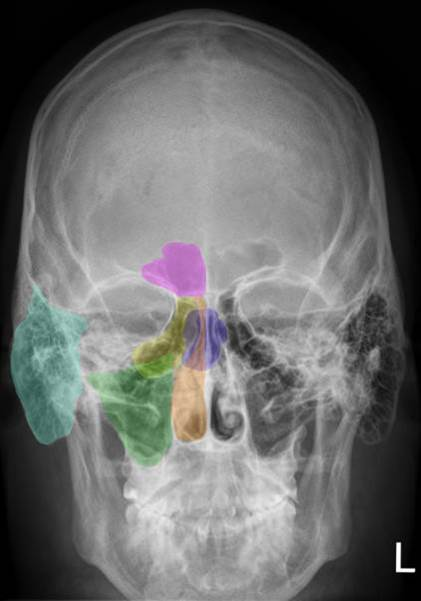
\includegraphics[width=.8\linewidth]{Bild2.jpg}
				\end{figure}
                \begin{figure}
                	\vspace*{-0.95cm}
                    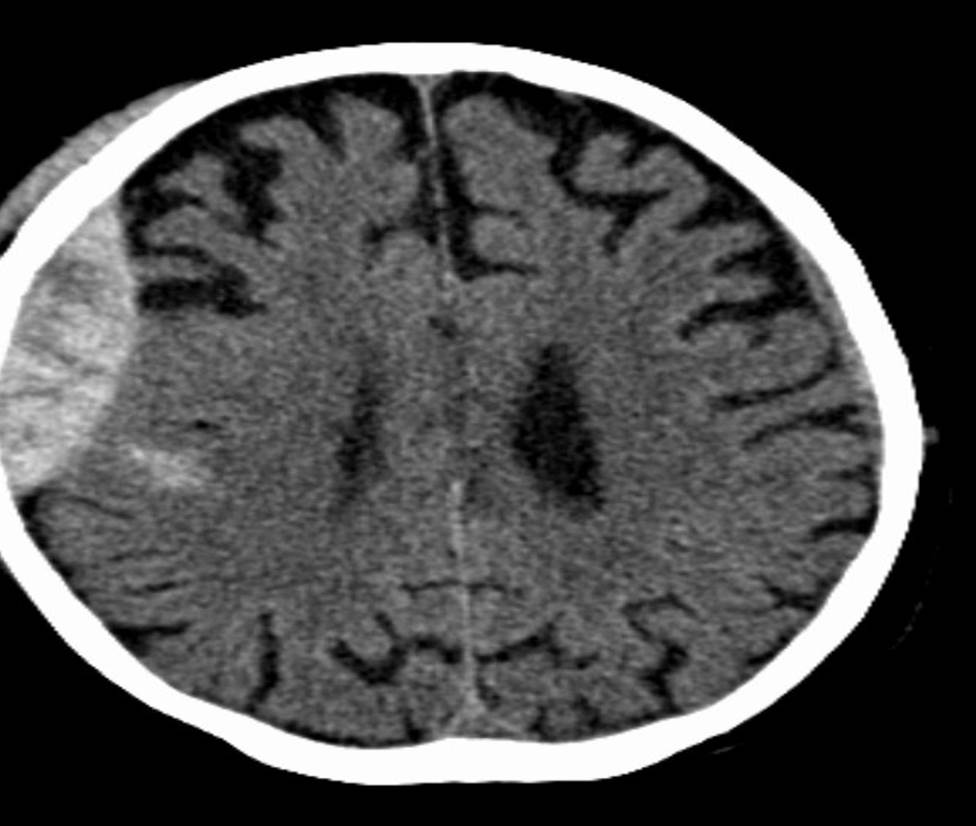
\includegraphics[width=.8\linewidth]{Bild3.jpg}
				\end{figure}
                \end{multicols}
                
                \begin{figure}
                    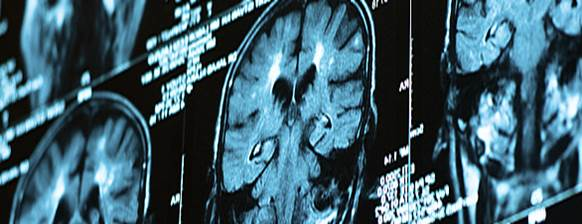
\includegraphics[width=.9\linewidth]{Bild4.jpg}
				\end{figure}
                
		\end{block}
      \end{column}
      
      \begin{column}{\sepmargin} \end{column}
      \end{columns} 
       
      \begin{columns}[t] % Split up the two columns wide column again
      
      \begin{column}{\sepmargin} \end{column}
        \begin{column}{\onecolwid} % The first column
			\begin{block}{\large Acknowledgements}
                    \begin{center}
						\begin{tabular}{SL}
							
\includegraphics[width=\linewidth]{Flag_of_Europe.png}  &
							\footnotesize This project has received funding from the  grant agreement No 11111.
						\end{tabular}
					\end{center}
				\end{block}	
                \vspace*{-0.9cm}
				\begin{alertblock}{\large Contact Information}
                \vspace*{-0.5cm}
					\begin{footnotesize}
					\begin{itemize}
						\item \href{mailto:email@meduniwien.ac.at}{email@meduniwien.ac.at}
						\item \href{http://www.example.com/}{www.example.com} - \href{www.meduniwien.ac.at/medstat}{www.meduniwien.ac.at/medstat}
					\end{itemize}
					\end{footnotesize}	
					
				\end{alertblock}
		    \end{column} % End of the first column
			\begin{column}{\sepwid}\end{column} % Empty spacer column
			\begin{column}{\onecolwid} % Begin a column 
              \begin{block}{\large References}
			  \vspace*{-0.5cm}
              	\nocite{*} % Insert publications even if they are not cited in the poster
					{\footnotesize
                    	%\bibliographystyle{plainurl}
						\bibliography{bibliog.bib}}
				\end{block} 
			\end{column} % End of the second column
            
			\begin{column}{\sepmargin}\end{column} % Empty spacer column
            
\end{columns} % End of all the columns in the poster


\end{frame} % End of the enclosing frame
	
\end{document}
